\documentclass[12pt,twocolumn,letterpaper]{article}

\usepackage{cvpr}
\usepackage{times}
\usepackage{epsfig}
\usepackage{graphicx}
\usepackage{amsmath}
\usepackage{amssymb}
\usepackage[breaklinks=true,bookmarks=false]{hyperref}
\usepackage{gensymb}
\usepackage{subcaption}

\cvprfinalcopy

\def\httilde{\mbox{\tt\raisebox{-.5ex}{\symbol{126}}}}


\setcounter{page}{1}
\begin{document}

\title{Visual Odometry on Smartphone}

\author{Jai Prakash\\
Carnegie Mellon University\\
Master of Science in Computer Vision\\
{\tt\small jprakash@andrew.cmu.edu}
\and
Utkarsh Sinha\\
Carnegie Mellon University\\
Master of Science in Computer Vision\\
{\tt\small usinha@andrew.cmu.edu}
}

\maketitle

\begin{abstract}
In this project, we are trying to localize the camera using visual odometry. The major component of the project is to generate keyframes according to pre-defined heuristics and triangulate the points to create 3D reconstruction of the scene. The intermediate frames can be found using Perspective-n-point algorithm. In addition, we also perform local bundle adjustment over last few frames so that the localization is locally consistent. We also plan to exploit the onboard inertial sensors to get prior for the localization.
\end{abstract}

\section{Introduction}

Augmented reality has been around for years, yet not all problems are solved in that domain. One of the challenges being precise localization of the device in the world. Most of the augmented reality applications on smartphones are based on markers. One good example of marker-based AR is Vuforia. On the other hand, there are standalone devices like Hololens, which has number of sensors to understand the scene and localize the head mounted display in the scene.

In many of the Augmented Reality application, you do not have to understand the scene. Sometimes, just localizing the camera in the world would solve the problem. In this project we focus on localizing the phone using the camera and the inertial sensors.

\section{Background}
\textbf{Visual SLAM vs. Visual Odometry: } The focus in the visual SLAM techniques is both in reconstruting the scene and also localizing the camera in the scene. However, our main focus is just in localization of the camera. For the scope of the project, we focus only to be locally consistent. So, our system might intrduce drift over time.


\section{Method}
Our system contains of the following blocks.
\begin{itemize}
\item \textbf{Feature Extraction and matching: } We have experimented with OpenCV KLT features, AKAZE features and ORB features. The KLT features can also be used for tracking the features in the subsequent frames. 
\end{itemize}

\begin{figure}
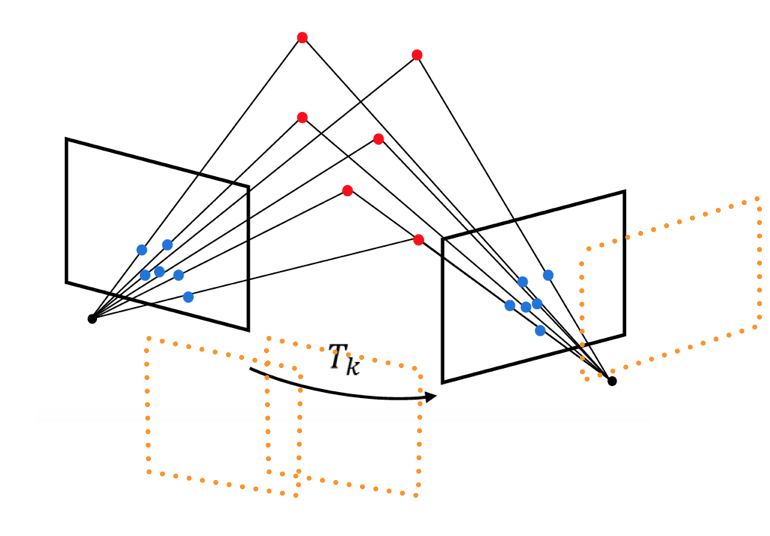
\includegraphics[width=0.5\textwidth]{images/system}
\caption{A visualization of the Visual Odometry system}
\label{fig:system}
\end{figure}

\begin{figure}
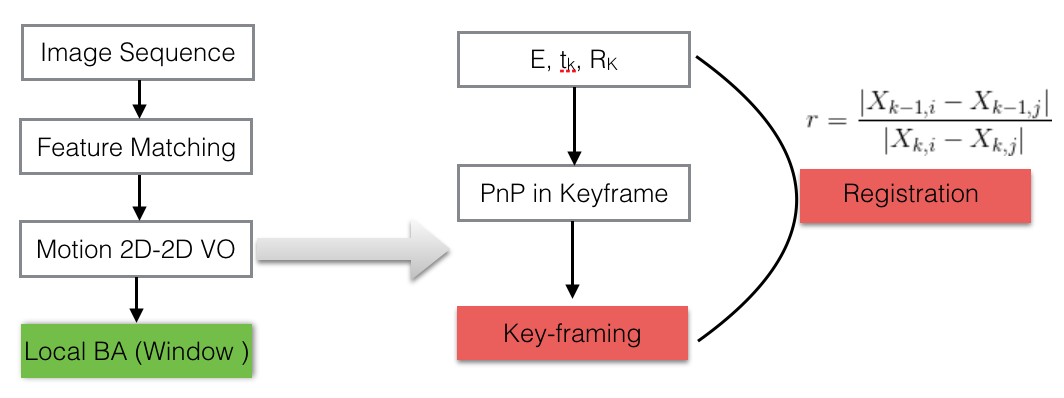
\includegraphics[width=0.5\textwidth]{images/block}
\caption{Block diagram of the system. The red blocks are implemented as a part of Geometry based vision project. For this project we are focusing on implementation of local bundle adjustment shown in green}
\label{fig:block}
\end{figure}


\section{Results}
So far, we have been working with the datasets available online. The results are illustrated on the Middlebury Temple dataset \cite{middlebury}. We are able to recosntruct the temple structure using the two keyframes (handpicked for now). Once the reconstruction is done, we are able to recover the camera poses as illustrated in the figure xxx



\section{Future Work}
\begin{itemize}
\item Evaluation of various features. 
\item Integration of inertial sensor in the pipeline
\item Integration of Google Ceres-solver for bundle adjustment.
\end{itemize}

    
{\small{
\begin{thebibliography}{15}

\bibitem{Szeliski}
Szeliski, Richard. \textit{Computer Vision: Algorithms and Applications}. 1st ed. London: Springer-Verlag, 2010. Print.

\bibitem{middlebury} 
Temple dataset \url{http://vision.middlebury.edu/mview/data/}

\endgroup
\end{document}